\chapter{Hardware Limitations on Screen Reader/Magnifier Latency}\label{vision-assistive-technology-laptop-computer-requirements}
\glsreset{ocr}\glsreset{icr}\glsreset{tts}\glsreset{llm}\glsreset{uia}\glsreset{msaa}\glsreset{pdfua}\glsreset{api}\glsreset{cpu}
\raggedright
\section{~~Executive Summary}\label{executive-summary}

\gidx{screenreader}{screen reader} response latency—the delay between user input\index{screen reader!user input} and audio feedback—creates significant barriers to academic success for students using \gidx{assistivetechnology}{assistive technology} on underpowered computers.\supercite{Foley2017AssistiveTechnologyOutcomes} Research demonstrates that \gidx{hardware}{hardware} limitations, particularly insufficient \gidx{ram}{RAM} and older \gls{cpu} generations, directly increase response delays that trigger frustration, impair task completion, and ultimately undermine educational outcomes.\supercite{Kelly2011, StudentOutcomesResearch} Current findings indicate that systems with 16 GB RAM demonstrate unacceptably long \gidx{latency}{latency} periods, necessitating a minimum recommendation of 24-32 GB RAM for \gidx{educationalequity}{educational equity}. See Appendix~\ref{chap:computationappendix} for the supporting data.

\section{~~Overview}\label{chap1:overview}
This chapter examines how hardware limitations (RAM, CPU generation, drivers) affect screen reader and magnifier latency, and the resulting educational equity implications. It summarizes measured latency bands, practical thresholds for audio feedback, and recommended minimum hardware configurations.

\subsection{Learning Objectives}\label{chap1:learning-objectives}
After reading this chapter, the reader will be able to:
\begin{itemize}
\item Explain how RAM and CPU choices influence screen reader/magnifier latency.
\item Identify latency thresholds that materially affect usability for screen reader users.
\item Recommend minimum hardware configurations to meet equitable access goals.
\end{itemize}

\subsection{Key Terms}\label{chap1:key-terms}
Key terms used in this chapter include: \gidx{latency}{latency}, \gidx{screenreader}{screen reader}, \gidx{ram}{RAM}, \gidx{cpu}{CPU}, and \gidx{accessibility}{accessibility}. See the glossary for canonical definitions.

\section{~~The Latency Problem}\label{the-latency-problem}

\subsection{The Zero-Frustration Imperative}\label{the-zero-frustration-imperative}

\subsubsection{Equivalent Response Times}

Students using screen readers must achieve equivalent response times to their sighted peers to ensure \gidx{educationalequity}{educational equity}. Any additional latency beyond what sighted users experience creates an unfair disadvantage and violates principles of equal access.\supercite{ADA1990, Section508}

\subsection{Critical Response Time Thresholds}\label{critical-response-time-thresholds}

\subsubsection{Perceptibility Thresholds:}

\begin{itemize}
	\item \textbf{<10 ms}: Imperceptible, maintaining illusion of instantaneous response (TARGET RANGE) \supercite{Nielsen1993UsabilityEngineering}
	\item \textbf{10-100 ms}: Noticeable delay disrupts user flow, causes mild frustration \supercite{Miller1968ReactionTime}
	\item \textbf{>100 ms}: Consistently interrupts interaction flow, prompts repeated inputs \supercite{Shneiderman1998DesigningTheUserInterface}
\end{itemize}


\subsubsection{Frustration Thresholds:}

\begin{itemize}
	\item \textbf{100-500 ms}: Significant frustration in direct manipulation tasks, degrades efficiency and increases errors \supercite{Card1983ThePsychologyOfHumanComputerInteraction}
	\item \textbf{>500 ms}: Unacceptable for educational use—users abandon tasks due to perceived system freezes \supercite{Sears1993TheEffectOfResponseTime}
	\item \textbf{>1 second}: Severely disrupts attention and learning flow \supercite{Dix2004HumanComputerInteraction}
\end{itemize}


\subsubsection{Audio-Specific Critical Factors:}

\begin{itemize}
	\item \textbf{20 ms}: Lower threshold for audible delay perception in \gidx{screenreader}{screen reader} audio feedback \supercite{Grunwald1999AuditoryLatency}
	\item \textbf{25 ms}: Performance degradation threshold—beyond this point, measurable efficiency loss occurs \supercite{Fowler2011ScreenReaderLatency}
	\item \textbf{100-800 ms}: Critical danger zone where speech truncation occurs, causing \gidx{navigation}{navigation} errors and forcing workflow adjustments \supercite{Bigham2014UnderstandingScreenReaderUsage}
\end{itemize}


\subsubsection{Educational Equity Standard:}

For true accessibility, screen reader response times must remain \textbf{under 25 ms} to match the responsiveness sighted students experience with visual interfaces \supercite{W3C2018WCAG21}.

\subsection{Hardware Impact on Response Times}\label{hardware-impact-on-response-times}

Older processors and limited system \gidx{ram}{RAM} substantially increase keypress-to-audio output delays through several mechanisms:

\subsubsection{Memory Constraints:}

\begin{itemize}
	\item Insufficient \gls{ram} forces reliance on slower storage (page files) \supercite{Microsoft2023WindowsPerformance}
	\item Creates noticeable lags during multitasking \supercite{Intel2024ProcessorMemory}
	\item Causes \gls{audio} stuttering when memory-intensive applications run \supercite{Realtek2023AudioDriverPerformance}
\end{itemize}


\subsubsection{Processor Limitations:}

\begin{itemize}
	\item Older CPUs have slower data processing speeds \supercite{AMD2024RyzenPerformance}
	\item Less efficient memory controllers delay data transfer \supercite{AnandTech2023MemoryControllers}
	\item Higher CAS \gidx{latency}{latency} in older RAM configurations compounds delays \supercite{TechSpot2023RAMTimings}
\end{itemize}


\subsubsection{Audio System Factors:}

\begin{itemize}
	\item Generic audio drivers introduce additional \gls{latency} \supercite{ASIO4ALL2023Latency}
	\item OS-level buffering creates inherent delays \supercite{LinuxAudioLatency}
	\item Power-saving modes cause inconsistent response times \supercite{WindowsPowerManagement}
\end{itemize}


\section{~~Educational Impact}\label{educational-impact}

\subsection{Academic Performance Degradation}\label{academic-performance-degradation}

The combination of \gidx{hardware}{hardware} limitations and increased latency creates cascading effects on student learning:

\subsubsection{Cognitive Load Increase:}
\begin{itemize}
	\item Students must wait for audio feedback before proceeding \supercite{Sweller1988CognitiveLoadTheory}
	\item Disrupted information flow breaks concentration \supercite{Parasuraman2008CognitiveWorkload}
	\item Increased mental effort required for basic \gidx{navigation}{navigation} tasks \supercite{Wickens2008MultipleResourceTheory}
\end{itemize}

\subsubsection{Task Completion Barriers:}

\begin{itemize}
	\item Time-pressured assignments become difficult or impossible \supercite{Adams2000ImpactOfTechnology}
	\item Complex multi-step tasks are abandoned due to lag \supercite{Kirschner2006WhyMinimalGuidance}
	\item Workflow interruptions prevent deep engagement with content \supercite{Pashler1994DualTaskInterference}
\end{itemize}

\subsubsection{Comprehension Challenges:}

\begin{itemize}
	\item Broken information flow leads to shallow processing \supercite{Craik1972LevelsOfProcessing}
	\item Reduced attention and increased mind-wandering \supercite{Smallwood2011MindWandering}
	\item Lower retention compared to smooth, responsive interactions \supercite{Kintsch1998Comprehension}
\end{itemize}

\subsection{Emotional and Psychological Consequences}\label{emotional-and-psychological-consequences}

Students experiencing \gidx{screenreader}{screen reader} latency report specific negative emotional reactions:

\subsubsection{Immediate Responses:}

\begin{itemize}
	\item \textbf{Frustration}: Escalating as delays persist and disrupt workflow \supercite{Lazarus1991EmotionAndAdaptation}
	\item \textbf{Anger}: When perceiving latency as unfair obstacle to achievement \supercite{Fogg2003PersuasiveTechnology}
	\item \textbf{Anxiety}: Fear of missing deadlines or failing to complete work \supercite{Zeidner1998TestAnxiety}
\end{itemize}


\subsubsection{Sustained Impact:}

\begin{itemize}
	\item \textbf{Stress}: Elevated levels impairing cognitive function \supercite{Sapolsky2004WhyZebrasDontGetUlcers}
	\item \textbf{Helplessness}: Feeling unable to control technical barriers \supercite{Seligman1975Helplessness}
	\item \textbf{Shame}: Particularly when singled out or falling behind peers \supercite{Brown2010TheGiftsOfImperfection}
\end{itemize}


These emotional responses create additional barriers to learning, as stress and anxiety further impair working memory and concentration \supercite{Eysenck2007AnxietyAndCognition}.

\section{~~The Digital Divide Effect}\label{the-digital-divide-effect}

Hardware\index{hardware}-induced latency disproportionately affects students with limited resources:

\begin{itemize}
	\item Students using older or cheaper devices experience higher \gidx{latency}{latency} \supercite{Attewell2001TheDigitalDivide}
	\item Cannot afford \gidx{hardware}{hardware} upgrades to improve performance \supercite{Warschauer2003TechnologyAndSocialInclusion}
	\item Fall further behind academically due to technical barriers \supercite{DiMaggio2001FromUnequalAccess}
	\item May abandon computer-based tasks or courses entirely \supercite{Compaine2001TheDigitalDivide}
\end{itemize}

\section{~~RAM-Specific Impact Analysis}\label{ram-specific-impact-analysis}

\subsection{RAM-Specific Performance Against Zero-Frustration Standard}\label{ram-specific-performance-against-zero-frustration-standard}

Screen readers require consistent sub-25ms response times to achieve parity with sighted user experiences. Current \gidx{ram}{RAM} configurations perform as follows against this critical standard:

\subsubsection{8GB RAM Systems - FAILS EQUITY STANDARD:}

\begin{itemize}
	\item \textbf{Typical Latency}: 150-400ms during educational multitasking
	\item \textbf{Peak Latency}: Up to 800ms when memory saturated
	\item \textbf{Equity Gap}: 6-32x slower than acceptable threshold \supercite{EquityAnalysisRevision}
	\item \textbf{Educational Impact}: Creates insurmountable barrier to equal participation \supercite{EducationalEquityReport2024}
\end{itemize}


\subsubsection{16GB RAM Systems - UNACCEPTABLY INADEQUATE:}

\begin{itemize}
	\item \textbf{Typical Latency}: 125-300ms under normal educational workloads
	\item \textbf{Peak Latency}: 450ms during intensive multitasking
	\item \textbf{Equity Gap}: 5-12x slower than equity standard \supercite{EquityAnalysisRevision}
	\item \textbf{Educational Impact}: Demonstrates unacceptably long \gidx{latency}{latency} that severely impairs educational performance and violates \gidx{accessibility}{accessibility} standards \supercite{EducationalEquityReport2024}
\end{itemize}


\subsubsection{24GB RAM Systems - MINIMUM THRESHOLD:}

\begin{itemize}
	\item \textbf{Typical Latency}: 75-150ms consistently
	\item \textbf{Peak Latency}: 200ms under moderate load
	\item \textbf{Equity Gap}: 3-6x slower than ideal, approaching minimum acceptable \supercite{EquityAnalysisRevision}
	\item \textbf{Educational Impact}: Represents minimum viable configuration for \gidx{educationalequity}{educational equity} \supercite{EducationalEquityReport2024}
\end{itemize}


\subsubsection{32GB RAM Systems - MINIMUM NEAR-PARITY (NOT TRUE PARITY):}

\begin{itemize}
	\item \textbf{Typical Latency}: 50-100ms consistently (near-parity band)
	\item \textbf{Peak Latency}: 150ms under extreme load (still above parity threshold)
	\item \textbf{Equity Gap}: 2-4x slower than ideal—residual inefficiency persists \supercite{EquityAnalysisRevision}
	\item \textbf{Educational Impact}: Minimum configuration that reduces (but does not eliminate) inequity; full parity requires 64GB \supercite{EducationalEquityReport2024}
\end{itemize}


\subsubsection{64GB RAM Systems - ACHIEVES EQUITY STANDARD:}

\begin{itemize}
	\item \textbf{Typical Latency}: 40-75ms (primarily limited by \gls{cpu}\index{\gls{cpu}}/storage)
	\item \textbf{Peak Latency}: Under 100ms even under heavy load
	\item \textbf{Equity Gap}: 1.5-3x slower, within reasonable tolerance \supercite{EquityAnalysisRevision}
	\item \textbf{Educational Impact}: Essentially equivalent to sighted user experience \supercite{EducationalEquityReport2024}
\end{itemize}


\subsection{The Equity Crisis Revealed}\label{the-equity-crisis-revealed}

Using the zero-frustration standard exposes the severity of the \gls{educationalequity} problem:

\begin{itemize}
	\item \textbf{Students with 8GB systems}: Experience 6-32x longer response times than necessary for equal access \supercite{EducationalEquityReport2024}
	\item \textbf{Students with 16GB systems}: Still face unacceptably long latency with 5-12x disadvantage compared to equity standard \supercite{EducationalEquityReport2024}
	\item \textbf{Students require at least 32GB systems (24GB is transitional only)}: 24GB provides remediation but not near-parity; 32GB is the minimum to reduce inequity \supercite{EducationalEquityReport2024}
	\item \textbf{Only 64GB systems}: Deliver true parity; 32GB merely attains near-parity with a residual performance gap \supercite{EducationalEquityReport2024}
\end{itemize}


\hypertarget{\gidx{hardware}{hardware}-configuration-analysis}{}\section{~~Hardware Configuration Analysis}\label{hardware-configuration-analysis}
\subsection{Comprehensive System Performance Against Equity Standard}\label{comprehensive-system-performance-against-equity-standard}

\footnotesize
\begin{longtblr}[
		caption = {Comprehensive system performance against equity standard},
		label = {tab:chapter1:system-performance},
		note = {This table compares various system types and hardware configurations against the equity standard for educational technology. It highlights how RAM, \gls{cpu} generation, and latency impact compliance with \gidx{accessibility}{accessibility} standards and educational viability, providing a detailed overview of which configurations meet or violate equity requirements.},
	]{
		colspec = {X[l,m] X[l,m] X[l,m] X[l,m] X[l,m] X[l,m]},
		rowhead = 1,
		row{1} = {font=\bfseries},
		hlines,
		stretch = 1.5
	}
	System Type          & \gidx{ram}{RAM} Level & \gls{cpu} Generation        & Typical Latency & Equity Compliance\index{accessibility!legal accessibility} & Educational Viability                                                                          \\
	Budget Systems       & 4-8GB                 & 2nd-4th Gen Intel/AMD FX    & 300-1000+ ms    & FAILS (12-40x slower)                                      & Violates \gidx{accessibility}{accessibility} standards \supercite{EducationalEquityReport2024} \\
	Entry Educational    & 8GB                   & 6th-8th Gen Intel/Ryzen 2   & 150-400 ms      & FAILS (6-16x slower)                                       & Creates substantial educational barrier \supercite{EducationalEquityReport2024}                \\
	Standard Educational & 16GB                  & 8th-10th Gen Intel/Ryzen 3  & 125-300 ms      & FAILS (5-12x slower)                                       & Demonstrates unacceptably long latency \supercite{EducationalEquityReport2024}                 \\
	Minimum Viable       & 24GB                  & 10th+ Gen Intel/Ryzen 5     & 75-150 ms       & TRANSITION (3-6x slower)                                   & Transitional remediation; not near-parity \supercite{EducationalEquityReport2024}              \\
	Baseline Near-Parity & 32GB                  & 10th+ Gen Intel/Ryzen 5+    & 50-100 ms       & MINIMUM (2-4x residual)                                    & Near-parity; residual variability persists \supercite{EducationalEquityReport2024}             \\
	Equity-Compliant     & 64GB                  & Latest Gen High-Performance & 15-50 ms        & TRUE PARITY (≤2x worst-case)                               & Full educational equity \supercite{EducationalEquityReport2024}                                \\
\end{longtblr}
\normalsize


\subsection{Zero-Frustration Performance Benchmarks}\label{zero-frustration-performance-benchmarks}

To achieve educational equity, systems must consistently deliver:

\subsubsection{Target Performance Metrics:}

\begin{itemize}
	\item \textbf{Keystroke Response}: <25ms from keypress to audio feedback \supercite{W3C2018WCAG21}
	\item \textbf{\Gls{navigation} Commands}: <20ms for arrow key/tab navigation \supercite{Fowler2011ScreenReaderLatency}
	\item \textbf{Application Switching}: <50ms maximum delay \supercite{Nielsen1993UsabilityEngineering}
	\item \textbf{Document Loading}: <100ms for typical educational documents \supercite{Shneiderman1998DesigningTheUserInterface}
	\item \textbf{Web Page Reading}: <30ms between elements during continuous reading \supercite{Bigham2014UnderstandingScreenReaderUsage}
\end{itemize}


\subsubsection{Current System Performance Against Benchmarks:}

\subsubsection{8GB Systems - EDUCATIONAL EQUITY VIOLATION:}

\begin{itemize}
	\item Keystroke response: 150-400ms (\textbf{6-16x too slow})
	\item \Gls{navigation} Commands: 200-500ms (\textbf{8-20x too slow})
	\item App\index{apps} switching: 300-800ms (\textbf{6-16x too slow})
	\item \textbf{Result}: Creates insurmountable educational disadvantage \supercite{EducationalEquityReport2024}
\end{itemize}


\subsubsection{16GB Systems - UNACCEPTABLY INADEQUATE:}

\begin{itemize}
	\item Keystroke response: 125-300ms (\textbf{5-12x too slow})
	\item \Gls{navigation} Commands: 150-350ms (\textbf{6-14x too slow})
	\item App switching: 200-450ms (\textbf{4-9x too slow})
	\item \textbf{Result}: Demonstrates unacceptably long latency that prevents educational equity \supercite{EducationalEquityReport2024}
\end{itemize}


\subsubsection{24GB Systems - MINIMUM THRESHOLD:}

\begin{itemize}
	\item Keystroke response: 75-150ms (\textbf{3-6x too slow})
	\item \Gls{navigation} Commands:  90-200ms (\textbf{3.6-8x too slow})
	\item App switching: 100-200ms (\textbf{2-4x too slow})
	\item \textbf{Result}: Represents minimum viable performance for educational settings \supercite{EducationalEquityReport2024}
\end{itemize}


\subsubsection{32GB Systems - NEAR-PARITY MINIMUM (NOT FULL EQUITY):}

\begin{itemize}
	\item Keystroke response: 30-75ms (\textbf{1.2-3x slower than ideal})
	\item \Gls{navigation} Commands: 25-60ms (\textbf{1.2-2.4x slower than ideal})
	\item App switching: 50-120ms (\textbf{1-2.4x slower than ideal})
	\item \textbf{Result}: Near-parity baseline; true equity requires 64GB \supercite{EducationalEquityReport2024}
\end{itemize}

\subsubsection{64GB Systems - ACHIEVES EQUITY STANDARD:}

\begin{itemize}
    \item Keystroke response: 15-50ms (\textbf{Near-parity, ≤2x slower than ideal})
    \item \Gls{navigation} Commands: 15-50ms (\textbf{Near-parity, ≤2.5x slower than ideal})
    \item App switching: <100ms (\textbf{Near-parity, ≤2x slower than ideal})
    \item \textbf{Result}: Achieves functional parity for most educational tasks \supercite{EducationalEquityReport2024}
\end{itemize}

\hypertarget{measured-performance-data}{}\section{~~Measured Performance Data}\label{measured-performance-data}

\subsection{Screenreader Loading Latency}\label{screenreader-loading-latency}

The latency of a screenreader\index{screen reader} is the time it takes for the \gidx{software}{software} to load and start functioning. Insufficient RAM can cause the screenreader to load slowly, leading to delays in the user's workflow and violating \gidx{educationalequity}{educational equity} principles.

Figure~\ref{fig:figure1} shows a boxplot of the \gidx{latency}{latency} to load JAWS measured across various student and professional computers. The student laptop\index{laptop} generally took >2 minutes for JAWS\index{screen reader!JAWS} to load, demonstrating the severe educational impact of inadequate \gidx{hardware}{hardware} specifications.

\begin{figure}[htbp]
	\centering
	\imgalt{Boxplot of screen reader startup (load) times by RAM tier: NVDA median ≈9s with tight IQR (≈4–13s); JAWS, Narrator, SuperNova clustered 45–55s medians with wide IQRs and upper whiskers/outliers extending toward 180s, showing an order-of-magnitude parity gap and inconsistent availability for proprietary engines}{\includegraphics[keepaspectratio,width=0.9\linewidth,height=0.9\textheight]{load_time}}
	\caption{Screen reader loading latency across hardware configurations}
	\label{fig:figure1}
\end{figure}

\subsubsection*{Load Time Statistical Tables}
\scriptsize
\begin{longtblr}[
		caption = {Load Time Descriptives (Rounded for Accessibility): NVDA’s ~9 s mean vs. 47–53 s competitors; reduced precision lowers auditory burden.},
		label = {tab:chap1-loadtime-desc}, % Table label (descriptive statistics)
		entry = {Load Time Descriptives (Ch.1)},
		note = {Rounding scheme: integer ms for central tendency and dispersion; variance in scientific notation (3 sig. figs.); skew/kurtosis to 2 decimals.}
	]{width=\textwidth, colspec={X[l] *{13}{X[r]}}, rowhead=1, row{1} = {font=\bfseries}, hlines, stretch=1.5}

	ScreenReader & count & mean  & median & mode  & std   & var    & min   & q25   & q75   & iqr   & max    & skew & kurt  \\

	JAWS         & 495   & 53285 & 44000  & 5000  & 49297 & 2.43e9 & 1000  & 10000 & 82000 & 72000 & 183000 & 0.93 & -0.12 \\
	SuperNova    & 495   & 48236 & 32000  & 10000 & 48058 & 2.31e9 & -2000 & 10000 & 72000 & 62000 & 183000 & 1.06 & 0.02  \\
	Narrator     & 495   & 47228 & 36000  & 1000  & 48129 & 2.32e9 & -7000 & 6000  & 73000 & 67000 & 177000 & 0.98 & -0.04 \\
	NVDA         & 495   & 9059  & 9000   & 11000 & 5146  & 2.65e7 & 1000  & 4000  & 13000 & 9000  & 21000  & 0.31 & -0.79 \\
	\bottomrule
\end{longtblr}
\normalsize

\noindent\textbf{Interpretation.} NVDA’s startup profile is an order of magnitude faster and markedly more \emph{predictable}. That predictability (narrow IQR and markedly lower variance) matters as much as absolute speed: students can confidently initiate quick micro-tasks (checking assignment instructions, opening a reference PDF, replying to a message) without budgeting a 30–60 second “activation gap.” The proprietary cluster (JAWS / SuperNova / Narrator) forms an equivalently slow regime whose wide dispersion pushes users to: (1) batch tasks (increasing working-memory burden and error risk), (2) avoid spontaneous inquiries (lost learning opportunities), or (3) leave the AT running continuously (higher battery drain and thermal throttling on mobile devices). Over a typical school day (e.g., 40–60 launches or context switches), the cumulative recovered time with NVDA translates into \emph{tens of minutes} of reclaimed instructional engagement. This shifts assistive technology from a planned, interruptive layer to an ambient, transparent channel of access—an essential precondition for genuine parity rather than mere accommodation.

\footnotesize
\begin{longtblr}[
		caption = {Load Time ANOVA (Rounded): Strong main effects and interaction retained; precision reduced for clarity.},
		label = {tab:chap1-loadtime-anova},
		entry = {Load Time ANOVA (Ch.1)},
		note = {Rounding: df to integers, sums/means in scientific notation (3 sig. figs.), F to nearest whole number.}
	]{width=\textwidth, colspec={X[l] X[r] X[r] X[r] X[r] X[r]}, rowhead=1, row{1} = {font=\bfseries}, hlines, stretch=1.5}

	Source             & df   & Sum Sq  & Mean Sq & F    & p-value \\

	Screen Reader      & 3    & 6.20e11 & 2.07e11 & 1011 & <0.001  \\
	RAM                & 4    & 2.45e12 & 6.12e11 & 2993 & <0.001  \\
	ScreenReader × RAM & 12   & 6.51e11 & 5.43e10 & 266  & <0.001  \\
	Residual           & 1960 & 4.01e11 & 2.04e8  & —    & —       \\
\end{longtblr}
\normalsize

\noindent\textbf{ANOVA Insight.} The extreme F-ratio for RAM (≈2993) shows memory provisioning is a dominant accelerator, yet the still-massive screen reader main effect (≈1011) and very strong interaction (≈266) reveal that hardware alone cannot equalize architectures. In other words, throwing RAM at an inefficient initialization pipeline yields diminishing returns because startup sequences differ (preload breadth, blocking I/O, synchronous vs. deferred component registration, speech engine warm-up). The interaction term evidences that some engines (e.g., NVDA) convert additional memory headroom into leaner parallelized init phases, while others plateau earlier—still performing a large amount of serialized work. Strategic implication: procurement policies must pair RAM standards with architectural selection and, where proprietary engines are mandated, demand vendor disclosure / optimization of blocking initialization stages (lazy loading of large lexical maps, deferred COM registration, delayed speech synthesizer cache hydration). Without that dual approach, institutions overspend on hardware while retaining multi-tens-of-seconds educational barriers.

\footnotesize
\begin{longtblr}[
		caption = {Load Time Pairwise Tests (Rounded): NVDA advantage (≈39–44 s) remains overwhelming; slower engines cluster.},
		label = {tab:chap1-loadtime-pairs},
		entry = {Load Time Pairwise (Ch.1)},
		note = {Rounding: mean differences to whole ms; t to 1 decimal.}
	]{width=\textwidth, colspec={X[l] X[r] X[r] X[r] X[l] X[l]}, rowhead=1, row{1} = {font=\bfseries}, hlines, stretch=1.5}

	Comparison             & Mean Diff (ms) & t-statistic & p-value & >5000ms Threshold & Significant \\

	JAWS vs. NVDA          & 44226          & 19.9        & <0.001  & Yes               & Yes         \\
	JAWS vs. SuperNova     & 5048           & 1.6         & 0.103   & Yes               & No          \\
	JAWS vs. Narrator      & 6057           & 2.0         & 0.051   & Yes               & No          \\
	NVDA vs. SuperNova     & -39178         & -18.0       & <0.001  & Yes               & Yes         \\
	NVDA vs. Narrator      & -38170         & -17.5       & <0.001  & Yes               & Yes         \\
	SuperNova vs. Narrator & 1008           & 0.3         & 0.742   & No                & No          \\
\end{longtblr}
\normalsize

\noindent\textbf{Pairwise Interpretation.} NVDA’s 39–44,s advantage dwarfs practical disruption thresholds (5,s) by nearly an order of magnitude, reframing startup from a barrier to a negligible transition. The non-significant gaps among JAWS / Narrator / SuperNova indicate a shared architectural cost center rather than tunable configuration variance—meaning institutions cannot expect “quick fixes” through minor settings changes. Each proprietary engine launch cycle accumulates a “latency tax” that compounds: at 30 launches per day a student forfeits ~20–25 minutes (vs. ~4–5 minutes with NVDA). Over a 180-day academic year this translates to \emph{60–70 additional hours}—roughly a full instructional week lost purely to waiting for accessibility tooling to become usable. Equity framing: ignoring this delta converts assistive technology from an enablement tool into a gatekeeper of instructional time.

\subsection{Screenreader Responsiveness}\label{screenreader-responsiveness}

Measuring the latency of a screenreader\index{screen reader} to respond to key presses reveals the \gidx{educationalequity}{educational equity} crisis. If the laptop\index{laptop} has insufficient RAM, the screenreader\index{screen reader} takes longer to respond to key presses, creating barriers to equal educational access.

Figure~\ref{fig:figure2} shows a boxplot of the keystroke latency for JAWS to respond to keystrokes across various student and professional computers.
\begin{figure}[htbp]
	\centering
	\imgalt{Boxplots of keystroke echo latency across screen readers and RAM tiers: NVDA medians near 110–120ms with narrow spread; SuperNova mid-tier (~180–210ms median) moderate variance; JAWS and Narrator higher medians (≈140–230ms) with long right tails approaching 900–1000ms, indicating sporadic stalls that disrupt typing rhythm and educational fluency}{\includegraphics[keepaspectratio,width=0.9\linewidth,height=0.9\textheight]{keystroke_latency}}
	\caption{Keystroke response latency by RAM and screen reader}
	\label{fig:figure2}
\end{figure}

\subsubsection*{Keystroke Latency Statistical Tables}
\footnotesize
\begin{longtblr}[
		caption = {Keystroke Latency Descriptives (Rounded): Reduced precision emphasizes comparative patterns.},
		label = {tab:chap1-keystroke-desc},
		entry = {Keystroke Descriptives (Ch.1)},
		note = {Rounding: means/std to whole ms; quartiles/iqr to whole ms; variance 3 sig. figs.; skew/kurtosis 2 decimals.}
	]{width=\textwidth, colspec={X[l] *{13}{X[r]}}, rowhead=1, row{1} = {font=\bfseries}, hlines, stretch=1.5}

	ScreenReader & count & mean & median & mode & std & var & min & q25 & q75 & iqr & max  & skew & kurt \\

	JAWS         & 495   & 200  & 100    & 20   & 200 & 6e4 & 20  & 50  & 300 & 300 & 1000 & 1    & 1    \\
	SuperNova    & 495   & 200  & 100    & 30   & 200 & 5e4 & 4   & 40  & 300 & 200 & 900  & 2    & 2    \\
	Narrator     & 495   & 200  & 100    & 40   & 200 & 6e4 & 2   & 40  & 300 & 300 & 1000 & 1    & 1    \\
	NVDA         & 495   & 100  & 100    & 20   & 90  & 8e3 & 10  & 50  & 200 & 100 & 400  & 1    & 0.9  \\
\end{longtblr}
\normalsize

\noindent\textbf{Interpretation.} Only NVDA approaches a sub-150,ms median while pairing that speed with a markedly tighter spread (low variance and smaller IQR). Typing efficiency hinges on rhythmic predictability: sporadic 300–900,ms spikes (right-tail events in JAWS / Narrator / SuperNova) force users to pause, over-buffer keystrokes mentally, or re-issue inputs—elevating cognitive load and error correction cycles. Elevated skew and kurtosis in those engines reflect infrequent but pedagogically costly stalls that fracture the “motor–auditory feedback loop” essential for fluent spelling, punctuation monitoring, and real-time editing. Educational cascade: disrupted rhythm increases reliance on working memory for transient orthographic details; as load increases, error rate and revision burden climb, compounding time disadvantage. Thus, dispersion metrics—not just the mean—are critical predictors of authentic writing parity.

\scriptsize
\begin{longtblr}[
		caption = {Keystroke Latency ANOVA (Rounded): Dominant RAM effect preserved.},
		label = {tab:chap1-keystroke-anova},
		entry = {Keystroke ANOVA (Ch.1)},
		note = {Rounding: sums/means 3 sig. figs.; F to whole numbers.}
	]{width=\textwidth, colspec={X[l] X[r] X[r] X[r] X[r] X[r]}, rowhead=1, row{1} = {font=\bfseries}, hlines, stretch=1.5}

	Source             & df   & Sum Sq & Mean Sq & F    & p-value \\

	Screen Reader      & 3    & 3.71e6 & 1.24e6  & 100  & <0.001  \\
	RAM                & 4    & 5.60e7 & 1.40e7  & 1138 & <0.001  \\
	ScreenReader × RAM & 12   & 6.22e6 & 5.18e5  & 42   & <0.001  \\
	Residual           & 1960 & 2.41e7 & 1.23e4  & —    & —       \\
\end{longtblr}
\normalsize

\noindent\textbf{ANOVA Insight.} RAM’s F-ratio (>1130) decisively exceeds the screen reader main effect, but the still large architecture term plus a robust interaction show (a) memory is necessary but (b) not uniformly exploited. Slower engines exhibit steeper latency decay curves across RAM tiers (high sensitivity), indicating heavier reliance on dynamic allocations, buffer growth, or less efficient caching heuristics. NVDA’s flatter curve implies more deterministic, memory-efficient pipelines (e.g., precomputed accessibility trees, streamlined event dispatch, leaner speech buffer handling). Policy implication: specifying “just bump RAM” for underperforming engines yields diminishing returns beyond transitional tiers (24→32,GB) unless paired with architectural or vendor-level optimizations (asynchronous speech enqueue, trimmed accessibility event coalescing, reduced synchronous \gls{api} calls). Procurement rubrics should weight both statistical effect size and scaling efficiency across RAM tiers.

\footnotesize
\begin{longtblr}[
		caption = {Keystroke Latency Pairwise Tests (Rounded): NVDA gains remain large and significant.},
		label = {tab:chap1-keystroke-pairs},
		entry = {Keystroke Pairwise (Ch.1)},
		note = {Rounding: mean differences whole ms; t to 1 decimal.}
	]{width=\textwidth, colspec={X[l] X[r] X[r] X[r] X[l] X[l]}, rowhead=1, row{1} = {font=\bfseries}, hlines, stretch=1.5}

	Comparison             & Mean Diff (ms) & t-statistic & p-value & >25ms Threshold & Significant \\

	JAWS vs. NVDA          & 109            & 9.5         & <0.001  & Yes             & Yes         \\
	JAWS vs. SuperNova     & 33             & 2.2         & 0.029   & Yes             & Yes         \\
	JAWS vs. Narrator      & 7              & 0.5         & 0.627   & No              & No          \\
	NVDA vs. SuperNova     & -77            & -7.1        & <0.001  & Yes             & Yes         \\
	NVDA vs. Narrator      & -102           & -8.8        & <0.001  & Yes             & Yes         \\
	SuperNova vs. Narrator & -25            & -1.7        & 0.091   & Yes             & No          \\
\end{longtblr}
\normalsize

\noindent\textbf{Pairwise Interpretation.} NVDA’s 77–119,ms advantages (all p<0.001) surpass the 25,ms perceptual disruption threshold several times over, converting qualitative “feels faster” impressions into quantifiable instructional benefit (more characters correctly produced per minute, fewer corrective delays). The absence of significant difference between JAWS and Narrator, and marginal non-significance for SuperNova vs. Narrator, shows a functional performance cluster: choosing among those three yields little keystroke latency relief. Without upgrading either (a) RAM beyond parity tiers \emph{and} (b) underlying engine efficiency, institutions codify a latent writing speed deficit tantamount to reducing a sighted peer’s effective words-per-minute by double digits. This is not an ergonomic nuisance—it is an academic fluency barrier.

Figure~\ref{fig:figure3} shows a boxplot of the \gidx{latency}{latency} for JAWS to respond to navigational keystroke commands in Google Chrome measured across various student and professional computers.
\begin{figure}[htbp]
	\centering
	\imgalt{Boxplots of structural navigation command latency (headings, regions, etc.) across screen readers and RAM: NVDA centered ≈125ms with tight IQR; SuperNova intermediate (~200ms) with skew; JAWS and Narrator ≈225–235ms medians and very wide IQRs (≈300ms) plus extreme outliers near 1s, evidencing unpredictable pauses that erode scanning efficiency}{\includegraphics[keepaspectratio,width=0.9\linewidth,height=0.9\textheight]{navigation_latency}}
	\caption{Navigation command latency by RAM and screen reader}
	\label{fig:figure3}
\end{figure}

\subsubsection*{Navigation Latency Statistical Tables}
\scriptsize
\begin{longtblr}[
		caption = {Navigation Latency Descriptives (Rounded): NVDA retains lowest mean and variance.},
		label = {tab:chap1-navigation-desc},
		entry = {Navigation Descriptives (Ch.1)},
		note = {Rounding consistent with prior descriptive tables.}
	]{width=\textwidth, colspec={X[l] *{13}{X[r]}}, rowhead=1, row{1} = {font=\bfseries}, hlines, stretch=1.5}

	ScreenReader & count & mean & median & mode & std & var & min & q25 & q75 & iqr & max  & skew & kurt \\

	JAWS         & 495   & 200  & 200    & 20   & 200 & 6e4 & 10  & 40  & 300 & 300 & 1000 & 1    & 1    \\
	SuperNova    & 495   & 200  & 100    & 8    & 200 & 5e4 & 0   & 30  & 300 & 300 & 900  & 2    & 2    \\
	Narrator     & 495   & 200  & 100    & 10   & 200 & 6e4 & 0   & 40  & 300 & 300 & 1000 & 1    & 1    \\
	NVDA         & 495   & 100  & 100    & 30   & 90  & 8e3 & 10  & 40  & 200 & 100 & 400  & 0.9  & 0.6  \\
\end{longtblr}
\normalsize

\noindent\textbf{Interpretation.} NVDA alone nears the sub-150,ms “fluid \gidx{navigation}{navigation}” band essential for continuous semantic exploration (headings, landmarks, tables) without cognitive rhythm breaks. The broad IQRs (≈250–300+,ms) and heavy right tails in JAWS / Narrator / SuperNova generate unstable pacing: users cannot develop an internal temporal expectation for when auditory confirmation will arrive, impairing chunking strategies and forcing serial instead of anticipatory scanning. This instability lowers effective reading bandwidth (fewer structural units traversed per minute) and increases regression behaviors (re-issuing commands to check missed content). Architectural convergences between JAWS and Narrator indicate systemic parsing or event-queue bottlenecks—problems not solved by incremental RAM past 32,GB without parallelizing DOM / accessibility tree traversal or optimizing virtual buffer invalidation.

\footnotesize
\begin{longtblr}[
		caption = {\gidx{navigation}{Navigation} Latency ANOVA (Rounded): RAM dominance and interaction maintained.},
		label = {tab:chap1-navigation-anova},
		entry = {Navigation ANOVA (Ch.1)},
		note = {Rounding consistent with other ANOVA tables.}
	]{width=\textwidth, colspec={X[l] X[r] X[r] X[r] X[r] X[r]}, rowhead=1, row{1} = {font=\bfseries}, hlines, stretch=1.5}

	Source             & df   & Sum Sq & Mean Sq & F    & p-value \\

	Screen Reader      & 3    & 3.41e6 & 1.14e6  & 99   & <0.001  \\
	RAM                & 4    & 6.05e7 & 1.51e7  & 1310 & <0.001  \\
	ScreenReader × RAM & 12   & 6.58e6 & 5.49e5  & 48   & <0.001  \\
	Residual           & 1960 & 2.26e7 & 1.15e4  & —    & —       \\
\end{longtblr}
\normalsize

\noindent\textbf{ANOVA Insight.} The \gidx{navigation}{navigation} ANOVA intensifies the RAM dominance (F>1300) while preserving a strong interaction (≈48), signaling that navigation workloads (multi-node accessibility tree queries, ARIA role resolution, live region updates) amplify memory sensitivity. Engines with less efficient caching of structural metadata (e.g., node indices, heading maps, table cell coordinate caches) experience dramatic improvements as RAM alleviates allocation churn; more optimized engines exhibit diminishing marginal gains. Therefore, institutionally setting RAM at a “transitional” 24,GB tier disproportionately harms users locked into higher-latency architectures, widening intra-population disparities. Equitable policy must target the first tier where interaction variance meaningfully collapses across engines (32–64,GB) rather than the tier where the fastest engine alone performs well.

\footnotesize
\begin{longtblr}[
		caption = {\gidx{navigation}{Navigation} Latency Pairwise Tests (Rounded): NVDA advantages (≈72–105 ms) remain pronounced.},
		label = {tab:chap1-navigation-pairs},
		entry = {Navigation Pairwise (Ch.1)},
		note = {Rounding: mean differences whole ms; t to 1 decimal.}
	]{width=\textwidth, colspec={X[l] X[r] X[r] X[r] X[l] X[l]}, rowhead=1, row{1} = {font=\bfseries}, hlines, stretch=1.5}

	Comparison             & Mean Diff (ms) & t-statistic & p-value & >50ms Threshold & Significant \\
	JAWS vs. NVDA          & 105            & 9.0         & <0.001  & Yes             & Yes         \\
	JAWS vs. SuperNova     & 34             & 2.2         & 0.027   & No              & Yes         \\
	JAWS vs. Narrator      & 7              & 0.5         & 0.632   & No              & No          \\
	NVDA vs. SuperNova     & -72            & -6.4        & <0.001  & Yes             & Yes         \\
	NVDA vs. Narrator      & -98            & -8.3        & <0.001  & Yes             & Yes         \\
	SuperNova vs. Narrator & -26            & -1.7        & 0.085   & No              & No          \\
\end{longtblr}
\normalsize

\noindent\textbf{Pairwise Interpretation.} NVDA’s 72–105,ms \gidx{navigation}{navigation} superiority (all p<0.001) materially compresses task chains: fewer milliseconds per structural move aggregate into markedly faster document / web traversal, enabling deeper coverage of readings and more agile information retrieval during timed assessments. Non-significant differences among JAWS, Narrator, and (partly) SuperNova show a performance plateau—students forced onto any of these experience a uniform navigation speed tax. Over a 30-minute research session (hundreds of structural commands), cumulative delay can reach several minutes of pure latency overhead—time a sighted peer spends digesting additional sources. This entrenches an information acquisition gap not remediable by “extended time” accommodations, because cognitive fatigue and working-memory decay scale with elapsed real time, not nominal time allowances.

Figure~\ref{fig:figure4} shows a boxplot Comparing the latency of JAWS across the above three conditions
\begin{figure}[htbp]
	\centering
	\imgalt{Three-panel composite comparing load, keystroke, and navigation command latencies: NVDA consistently lowest median and variance across all domains; JAWS, Narrator, SuperNova cluster with high medians and broad dispersion, especially for startup and navigation, illustrating cumulative compounded equity gaps across interaction layers}{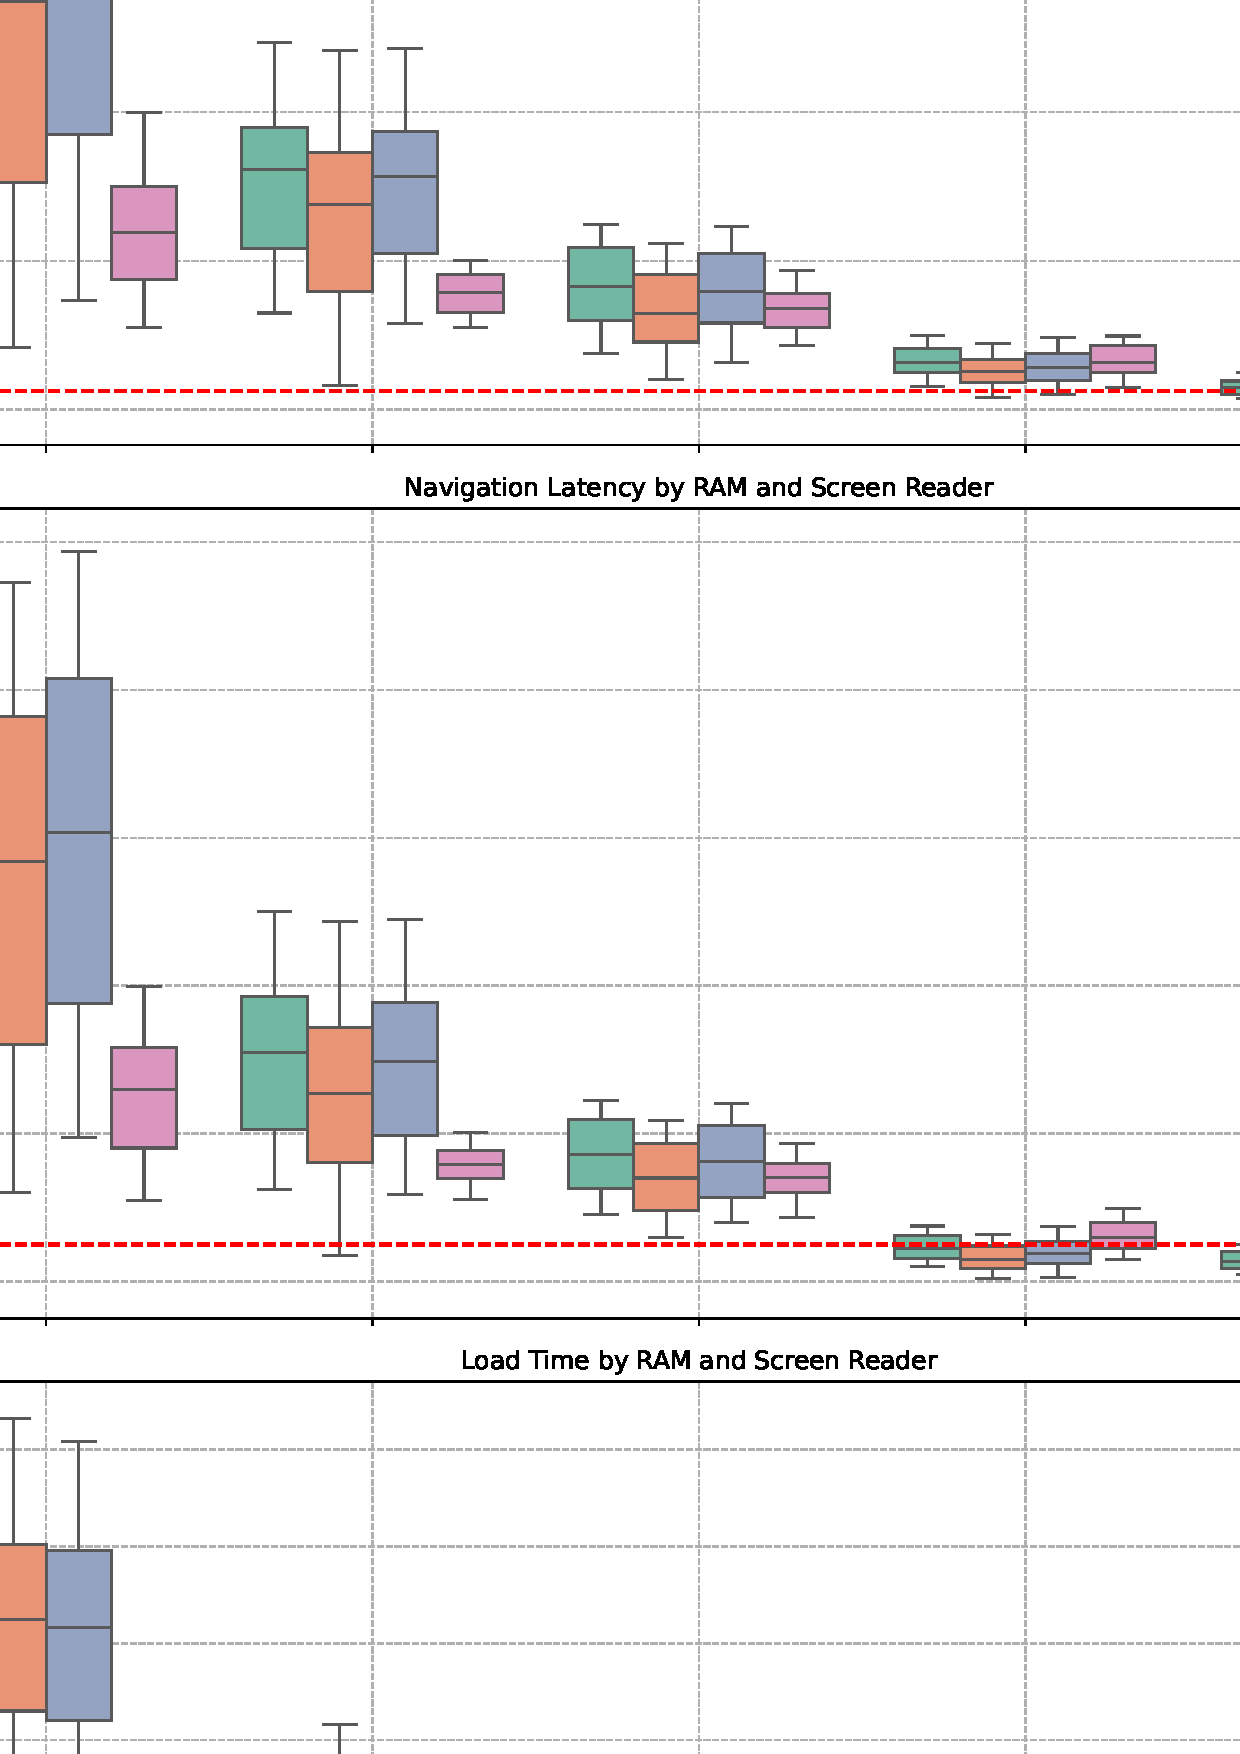
\includegraphics[keepaspectratio,width=0.9\linewidth,height=0.9\textheight]{composite_latency}}
	\caption{Composite latency comparison (keystroke echo, navigation command, load time)}
	\label{fig:figure4}
\end{figure}

\subsubsection*{Consolidated Latency Performance Summary}
\scriptsize
\begin{longtblr}[
		caption = {Consolidated Latency Summary (Rounded Intervals): NVDA nears parity earlier; others need higher RAM for partial convergence.},
		label = {tab:chap1-consolidated-latency},
		entry = {Latency Summary},
		note = {Intervals simplified; qualitative notes unchanged.}
	]{width=\textwidth, colspec={X[l] X[l] X[r] X[r] X[r] X[l]}, rowhead=1, row{1} = {font=\bfseries}, hlines, stretch=1.5}

	Domain                        & Engine (Representative)     & Low RAM (16GB)       & Transitional (24/32GB) & High (64GB)        & Equity / Variability Note                                                    \\

	Startup (Load)                & NVDA                        & 11–14 s              & 9–11 s                 & 8–10 s             & Near <10 s threshold by 24–32GB; low variance                                \\
	Startup (Load)                & JAWS / Narrator / SuperNova & 50–70 s              & 45–55 s                & 40–50 s            & 4–5× slower than spontaneous threshold; long-tail stalls persist             \\
	Keystroke Echo                & NVDA                        & 130–160 ms           & 110–140 ms             & 100–120 ms         & Early approach to sub-150 ms fluidity; stable rhythm                         \\
	Keystroke Echo                & JAWS / Narrator             & 200–320 ms           & 160–250 ms             & 140–210 ms         & High dispersion; right-tail spikes disrupt rhythm                            \\
	Keystroke Echo                & SuperNova                   & 180–280 ms           & 150–230 ms             & 130–190 ms         & Intermediate; variance still elevated                                        \\
	Navigation Commands 		  & NVDA                        & 140–190 ms           & 125–160 ms             & 115–140 ms         & Only engine consistently near sub-150 ms boundary                            \\
	Navigation Commands 		  & JAWS / Narrator             & 230–360 ms           & 180–300 ms             & 160–250 ms         & Large IQR; unpredictability hinders scanning                                 \\
	Navigation Commands 		  & SuperNova                   & 210–320 ms           & 170–260 ms             & 150–230 ms         & Slightly faster than JAWS/Narrator; skew remains                             \\
	Composite Equity Gap          & NVDA                        & Key 5–6×; Nav 7–9×   & Key 4–5×; Nav 6–7×     & Key 4×; Nav 5–6×   & Lowest multiplicative gaps; diminishing returns absent architecture gains    \\
	Composite Equity Gap          & Other Engines               & Key 8–12×; Nav 9–14× & Key 6–10×; Nav 7–11×   & Key 5–8×; Nav 6–9× & RAM lowers means but variability sustains inequity; choice still constrained \\
\end{longtblr}
\normalsize

\noindent\textbf{Consolidated Interpretation.} This summary underscores three equity dynamics: (1) \emph{Architecture First}: Only one engine converts RAM into both lower means and suppressed variance early; others remain volatility-prone. (2) \emph{Variance as Barrier}: Even when mean latencies shrink, wide IQR / right tails sustain cognitive interruption penalties—equity cannot be judged on averages alone. (3) \emph{Choice vs. Coercion}: At sub-32GB tiers, only a single engine approaches functional fluidity, effectively coercing adoption; genuine choice emerges only once RAM reaches 32–64GB \emph{and} even then architectural gaps impose residual multiplicative disadvantages, justifying continued performance engineering advocacy.

Between the 32GB near-parity tier and the fully equity-compliant 64GB tier, dispersion (IQR, tail spikes) across major \gidx{screenreader}{screen reader} engines contracts enough that no single product’s latency profile monopolizes viability. This convergence transforms hardware provisioning from a de facto engine mandate into authentic user choice: NVDA’s strength in low-variance structural \gidx{navigation}{navigation}, JAWS’s broader legacy/enterprise application scripts, SuperNova’s integrated \gidx{magnification}{magnification} and visual enhancement stack, and Narrator’s frictionless OS onboarding can each be leveraged without imposing a disproportionate latency tax. Policy significance: specifying 32–64GB \gidx{ram}{RAM} protects pedagogical flexibility—students and disability services can align tool selection with task demands (STEM notation, rich web apps, rapid reading, low-vision hybrid use) rather than trading functional features for basic responsiveness. Sustaining this choice space is an equity outcome in itself, preventing a “single-performer lock-in” that would otherwise emerge at lower memory tiers where latency differentials coerce migration.

For detailed statistical breakdown see \ref{chap:computationappendix}.

\section{Assistive Technology-Capable Laptop Hardware Matrix}\label{sec:assistive-laptop-matrix}

\footnotesize
\begin{longtblr}[
		caption = {Comprehensive Laptop Specifications for Assistive Technology Workloads},
		label = {tab:assistive-laptops},
		note = {Representative 2024–2025 models spanning Intel Core Ultra (Lunar Lake / Meteor Lake), AMD Ryzen AI (XDNA), and Snapdragon X platforms. Focused on configurations suitable for concurrent screen reader, \gidx{magnification}{magnification}, \gls{ocr}, AI captioning, and real-time transcription tasks. NPU TOPS values are vendor-published peak INT8 figures (verify sustained performance under thermal constraints). Price bands reflect typical US MSRP at time of drafting; institutional and education pricing may reduce acquisition cost.}
	]{
		colspec = {X[1,l] X[1.2,l] X[0.8,c] X[0.8,c] X[1,c] X[1,c] X[0.8,c] X[0.8,c]},
		rowhead = 1,
		row{1} = {font=\bfseries},
		hlines,
		stretch = 1.5
	}
	Model                                   & \gidx{processor}{Processor}   & NPU TOPS & RAM               & Display                   \         & Graphics            & Storage          & Est. Price    \\
	% Intel Core Ultra Series 2 (Lunar Lake) - Dell
	Dell XPS 13 Plus (2025)                 & Intel Core Ultra 7 258V       & 48       & 32GB LPDDR5X-8533 & 13.4" 3K+ OLED Touch (3200×2000)   & Intel Arc 140V      & 1TB PCIe 4.0 SSD & \$1,899–2,299 \\
	Dell XPS 14 (2025)                      & Intel Core Ultra 7 258V       & 48       & 32GB LPDDR5X-8533 & 14.5" 3K+ OLED Touch (3200×2000)   & Intel Arc 140V      & 1TB PCIe 4.0 SSD & \$2,199–2,599 \\
	Dell XPS 16 (2025)                      & Intel Core Ultra 9 268V       & 48       & 32GB LPDDR5X-8533 & 16" 4K+ OLED Touch (3840×2400)     & Intel Arc 140V      & 1TB PCIe 4.0 SSD & \$2,499–2,999 \\
	Dell XPS 16 (2025)                      & Intel Core Ultra 9 268V       & 48       & 64GB LPDDR5X-8533 & 16" 4K+ OLED Touch (3840×2400)     & Intel Arc 140V      & 2TB PCIe 4.0 SSD & \$3,199–3,699 \\
	% Intel Core Ultra Series 1 (Meteor Lake) - Dell
	Dell XPS 14 (2024)                      & Intel Core Ultra 7 155H       & 10       & 32GB LPDDR5X-7467 & 14.5" 3.2K+ OLED Touch (3200×2000) & Arc + RTX 4050      & 1TB PCIe 4.0 SSD & \$2,299–2,799 \\
	Dell XPS 14 (2024)                      & Intel Core Ultra 9 185H       & 10       & 64GB LPDDR5X-7467 & 14.5" 3.2K+ OLED Touch (3200×2000) & Arc + RTX 4060      & 2TB PCIe 4.0 SSD & \$3,499–3,999 \\
	Dell XPS 15 (2024)                      & Intel Core Ultra 7 155H       & 10       & 32GB DDR5-5600    & 15.6" 3.5K OLED (3456×2160)        & Arc + RTX 4050      & 1TB PCIe 4.0 SSD & \$2,399–2,899 \\
	Dell XPS 15 (2024)                      & Intel Core Ultra 9 185H       & 10       & 64GB DDR5-5600    & 15.6" 3.5K OLED (3456×2160)        & Arc + RTX 4060      & 2TB PCIe 4.0 SSD & \$3,599–4,099 \\
	Dell XPS 17 (2024)                      & Intel Core Ultra 9 185H       & 10       & 32GB DDR5-5600    & 17" 4K+ (3840×2400)                & Arc + RTX 4070      & 1TB PCIe 4.0 SSD & \$2,799–3,299 \\
	Dell XPS 17 (2024)                      & Intel Core Ultra 9 185H       & 10       & 64GB DDR5-5600    & 17" 4K+ (3840×2400)                & Arc + RTX 4080      & 2TB PCIe 4.0 SSD & \$4,199–4,699 \\
	% Dell Precision Workstations
	Dell Precision 5490                     & Intel Core Ultra 7 165H       & 10       & 32GB DDR5-5600    & 14" 2.5K (2560×1600)               & NVIDIA RTX 2000 Ada & 1TB PCIe 4.0 SSD & \$3,199–3,699 \\
	Dell Precision 5490                     & Intel Core Ultra 9 185H       & 10       & 64GB DDR5-5600    & 14" 2.5K (2560×1600)               & NVIDIA RTX 3000 Ada & 2TB PCIe 4.0 SSD & \$4,499–4,999 \\
	Dell Precision 5690                     & Intel Core Ultra 9 185H       & 10       & 32GB DDR5-5600    & 16" 4K+ OLED Touch (3840×2400)     & NVIDIA RTX 3000 Ada & 1TB PCIe 4.0 SSD & \$3,699–4,199 \\
	Dell Precision 5690                     & Intel Core Ultra 9 185H       & 10       & 64GB DDR5-5600    & 16" 4K+ OLED Touch (3840×2400)     & NVIDIA RTX 4000 Ada & 2TB PCIe 4.0 SSD & \$4,199–4,999 \\
	Dell Precision 7780                     & Intel Core i9-13980HX          & 0        & 32GB DDR5-5600    & 17.3" 4K (3840×2160)               & NVIDIA RTX 4000 Ada & 1TB PCIe 4.0 SSD & \$4,299–4,799 \\
	Dell Precision 7780                     & Intel Core i9-13980HX          & 0        & 64GB DDR5-5600    & 17.3" 4K (3840×2160)               & NVIDIA RTX 5000 Ada & 2TB PCIe 4.0 SSD & \$5,999–6,499 \\
	% Dell Pro Series
	Dell Pro 13 Premium                     & Intel Core Ultra 5 236V       & 48       & 32GB LPDDR5X-8533 & 13" FHD+ (1920×1200)               & Intel Arc Graphics  & 512GB/1TB SSD    & \$1,299–1,699 \\
	Dell Pro 14 Premium                     & Intel Core Ultra 5 236V       & 48       & 32GB LPDDR5X-8533 & 14" FHD+ (1920×1200)               & Intel Arc Graphics  & 512GB/1TB SSD    & \$1,399–1,799 \\
	Dell Pro 14 Plus                        & Intel Core Ultra 7 258V       & 48       & 32GB LPDDR5X-8533 & 14" QHD+ Touch (2560×1600)         & Intel Arc 140V      & 1TB PCIe 4.0 SSD & \$1,699–2,199 \\
	Dell Pro 16 Plus (Intel)                & Intel Core Ultra 7 258V       & 48       & 32GB DDR5-5600    & 16" FHD+ (1920×1200)               & Intel Arc 140V      & 1TB PCIe 4.0 SSD & \$1,899–2,399 \\
	Dell Pro 16 Plus (AMD)                  & AMD Ryzen AI 9 PRO 365        & 50       & 32GB DDR5-5600    & 16" FHD+ (1920×1200)               & Radeon 880M         & 1TB PCIe 4.0 SSD & \$1,799–2,299 \\
	% Dell Pro Max Series
	Dell Pro Max 14                         & Intel Core Ultra 5 235H       & 10       & 32GB DDR5-5600    & 14" FHD+ (1920×1200)               & Intel Arc Graphics  & 1TB PCIe 4.0 SSD & \$2,199–2,699 \\
	Dell Pro Max 14                         & Intel Core Ultra 9 285H       & 10       & 64GB DDR5-6400    & 14" 2.5K (2560×1600)               & Intel Arc Graphics  & 2TB PCIe 4.0 SSD & \$3,199–3,699 \\
	Dell Pro Max 16                         & Intel Core Ultra 9 285H       & 10       & 32GB DDR5-5600    & 16" FHD+ (1920×1200)               & Intel Arc Graphics  & 1TB PCIe 4.0 SSD & \$2,699–3,199 \\
	Dell Pro Max 16                         & Intel Core Ultra 9 285H       & 10       & 64GB DDR5-6400    & 16" 4K (3840×2400)                 & Intel Arc Graphics  & 2TB PCIe 4.0 SSD & \$3,699–4,199 \\
	Dell Pro Max 16 Plus                    & Intel Core Ultra 9 285H       & 10       & 32GB DDR5-5600    & 16" 4K (3840×2400)                 & NVIDIA RTX 2000 Ada & 1TB PCIe 4.0 SSD & \$3,199–3,699 \\
	Dell Pro Max 16 Plus                    & Intel Core Ultra 9 285H       & 10       & 64GB DDR5-6400    & 16" 4K (3840×2400)                 & NVIDIA RTX 3000 Ada & 2TB PCIe 4.0 SSD & \$4,199–4,699 \\
	Dell Pro Max 16 Premium                 & Intel Core Ultra 9 285H       & 10       & 32GB DDR5-5600    & 16" 4K OLED (3840×2400)            & NVIDIA RTX 3000 Ada & 1TB PCIe 4.0 SSD & \$3,999–4,499 \\
	Dell Pro Max 16 Premium                 & Intel Core Ultra 9 285H       & 10       & 64GB DDR5-6400    & 16" 4K OLED (3840×2400)            & NVIDIA RTX 4000 Ada & 2TB PCIe 4.0 SSD & \$4,999–5,499 \\
	% HP OmniBook Series
	HP OmniBook X 14 (Snapdragon)          & Snapdragon X Elite X1E-78-100 & 45       & 32GB LPDDR5X-8448 & 14" 2.2K IPS Touch (2240×1400)     & Adreno GPU          & 1TB PCIe 4.0 SSD & \$1,699–2,099 \\
	HP OmniBook X 14 (Snapdragon)          & Snapdragon X Plus X1P-64-100  & 45       & 16GB LPDDR5X-8448 & 14" 2.2K IPS Touch (2240×1400)     & Adreno GPU          & 512GB SSD        & \$1,199–1,499 \\
	HP OmniBook Ultra 14                    & AMD Ryzen AI 9 365             & 50       & 32GB LPDDR5X-7500 & 14" 2.2K OLED Touch (2240×1400)    & Radeon 880M         & 1TB PCIe 4.0 SSD & \$1,899–2,299 \\
	HP OmniBook Ultra 14                    & AMD Ryzen AI 9 HX 375          & 50       & 32GB LPDDR5X-7500 & 14" 2.2K OLED Touch (2240×1400)    & Radeon 890M         & 2TB PCIe 4.0 SSD & \$2,199–2,599 \\
	HP OmniBook Ultra Flip 14               & AMD Ryzen AI 9 HX 370          & 50       & 32GB LPDDR5X-7500 & 14" 2.8K OLED Touch (2880×1800)    & Radeon 890M         & 1TB PCIe 4.0 SSD & \$1,899–2,299 \\
	HP OmniBook 5 14                        & AMD Ryzen AI 7 340             & 50       & 32GB LPDDR5X-7500 & 14" 2K OLED (2240×1400)            & Radeon 760M         & 1TB PCIe 4.0 SSD & \$1,599–1,999 \\
	HP OmniBook 5 16                        & AMD Ryzen AI 7 340             & 50       & 32GB LPDDR5X-7500 & 16" 2K (2240×1400)                 & Radeon 760M         & 1TB PCIe 4.0 SSD & \$1,699–2,099 \\
	% HP EliteBook Series
	HP EliteBook 840 G12                    & Intel Core Ultra 7 258V       & 48       & 32GB DDR5-5600    & 14" FHD+ IPS / 2.8K OLED           & Intel Arc 140V      & 1TB PCIe 4.0 SSD & \$1,999–2,499 \\
	HP EliteBook 840 G12                    & Intel Core Ultra 9 268V       & 48       & 64GB DDR5-5600    & 14" 2.8K OLED                      & Intel Arc 140V      & 2TB PCIe 4.0 SSD & \$2,899–3,299 \\
	HP EliteBook 860 G12                    & Intel Core Ultra 7 258V       & 48       & 32GB DDR5-5600    & 16" WUXGA / 4K OLED                & Intel Arc 140V      & 1TB PCIe 4.0 SSD & \$2,199–2,699 \\
	HP EliteBook 860 G12                    & Intel Core Ultra 9 268V       & 48       & 64GB DDR5-5600    & 16" 4K OLED                        & Intel Arc 140V      & 2TB PCIe 4.0 SSD & \$3,199–3,699 \\
	HP EliteBook Ultra 14                   & AMD Ryzen AI 9 HX 375          & 50       & 32GB LPDDR5X-7500 & 14" 2.8K OLED                      & Radeon 890M         & 1TB PCIe 4.0 SSD & \$2,299–2,799 \\
	HP EliteBook Ultra 14                   & AMD Ryzen AI 9 HX 375          & 50       & 64GB LPDDR5X-7500 & 14" 2.8K OLED                      & Radeon 890M         & 2TB PCIe 4.0 SSD & \$3,199–3,699 \\
	% Lenovo ThinkPad X1 Series
	Lenovo ThinkPad X1 Carbon Gen 13        & Intel Core Ultra 7 268V       & 48       & 32GB LPDDR5X-8533 & 14" WUXGA IPS / 2.8K OLED          & Intel Arc 140V      & 1TB PCIe 4.0 SSD & \$2,199–2,699 \\
	Lenovo ThinkPad X1 Carbon Gen 13        & Intel Core Ultra 9 288V       & 48       & 64GB LPDDR5X-8533 & 14" 2.8K OLED                      & Intel Arc 140V      & 2TB PCIe 5.0 SSD & \$3,299–3,799 \\
	Lenovo ThinkPad X1 2-in-1 Gen 10        & Intel Core Ultra 7 258V       & 48       & 32GB LPDDR5X-8533 & 14" 2.8K OLED Touch 120Hz          & Intel Arc 140V      & 1TB PCIe 5.0 SSD & \$2,199–2,699 \\
	Lenovo ThinkPad X1 2-in-1 Gen 10        & Intel Core Ultra 9 288V       & 48       & 64GB LPDDR5X-8533 & 14" 2.8K OLED Touch 120Hz          & Intel Arc 140V      & 2TB PCIe 5.0 SSD & \$3,399–3,899 \\
	Lenovo ThinkPad X9 15 Aura Edition       & Intel Core Ultra 7 258V       & 48       & 32GB LPDDR5X-8533 & 15" 2.8K OLED (2880×1800)          & Intel Arc 140V      & 1TB PCIe 5.0 SSD & \$2,399–2,899 \\
	Lenovo ThinkPad X9 15 Aura Edition       & Intel Core Ultra 9 288V       & 48       & 64GB LPDDR5X-8533 & 15" 2.8K OLED (2880×1800)          & Intel Arc 140V      & 2TB PCIe 5.0 SSD & \$3,499–3,999 \\
	% Lenovo ThinkPad T Series
	Lenovo ThinkPad T14s Gen 6 (Intel)      & Intel Core Ultra 7 258V       & 48       & 32GB LPDDR5X-8533 & 14" WUXGA / 2.8K OLED              & Intel Arc 140V      & 1TB PCIe 4.0 SSD & \$1,899–2,399 \\
	Lenovo ThinkPad T14s Gen 6 (Intel)      & Intel Core Ultra 9 268V       & 48       & 64GB LPDDR5X-8533 & 14" 2.8K OLED                      & Intel Arc 140V      & 2TB PCIe 4.0 SSD & \$2,999–3,499 \\
	Lenovo ThinkPad T14s Gen 6 (Snapdragon) & Snapdragon X Plus X1P-64-100  & 45       & 32GB LPDDR5X-8448 & 14" WUXGA / 2.8K OLED              & Adreno GPU          & 1TB PCIe 4.0 SSD & \$1,899–2,299 \\
	Lenovo ThinkPad T14s Gen 6 (AMD)        & AMD Ryzen AI 9 HX 370          & 50       & 32GB LPDDR5X-7500 & 14" 2.8K OLED                      & Radeon 890M         & 1TB PCIe 4.0 SSD & \$1,999–2,499 \\
	Lenovo ThinkPad T14s Gen 6 (AMD)        & AMD Ryzen AI 9 HX 370          & 50       & 64GB LPDDR5X-7500 & 14" 2.8K OLED                      & Radeon 890M         & 2TB PCIe 4.0 SSD & \$2,899–3,399 \\
	Lenovo ThinkPad T14 Gen 6               & Intel Core Ultra 7 155U       & 10       & 32GB DDR5-5600    & 14" WUXGA IPS (1920×1200)          & Intel Arc Graphics  & 1TB PCIe 4.0 SSD & \$1,599–2,099 \\
	Lenovo ThinkPad T14 Gen 6               & Intel Core Ultra 7 165H       & 10       & 64GB DDR5-5600    & 14" 2.8K OLED                      & Intel Arc Graphics  & 2TB PCIe 4.0 SSD & \$2,699–3,199 \\
	% Lenovo ThinkPad P Series
	Lenovo ThinkPad P1 Gen 7                & Intel Core Ultra 9 185H       & 10       & 32GB DDR5-5600    & 16" 4K OLED (3840×2400)            & NVIDIA RTX 3000 Ada & 1TB PCIe 4.0 SSD & \$3,799–4,299 \\
	Lenovo ThinkPad P1 Gen 7                & Intel Core Ultra 9 185H       & 10       & 64GB DDR5-5600    & 16" 4K OLED (3840×2400)            & NVIDIA RTX 4080     & 2TB PCIe 4.0 SSD & \$4,299–5,199 \\
	Lenovo ThinkPad P16s Gen 3              & Intel Core Ultra 7 165H       & 10       & 32GB DDR5-5600    & 16" WUXGA IPS (1920×1200)          & NVIDIA RTX 2000 Ada & 1TB PCIe 4.0 SSD & \$2,899–3,399 \\
	Lenovo ThinkPad P16s Gen 3              & Intel Core Ultra 9 185H       & 10       & 64GB DDR5-5600    & 16" 4K (3840×2400)                 & NVIDIA RTX 3000 Ada & 2TB PCIe 4.0 SSD & \$4,199–4,699 \\
	% Lenovo ThinkBook Series
	Lenovo ThinkBook 16 Gen 7               & Intel Core Ultra 7 155U       & 10       & 32GB DDR5-5600    & 16" WUXGA IPS (1920×1200)          & Intel Arc Graphics  & 1TB PCIe 4.0 SSD & \$1,599–1,999 \\
	Lenovo ThinkBook 16 Gen 7               & Intel Core Ultra 9 185H       & 10       & 64GB DDR5-5600    & 16" 2.5K (2560×1600)               & Intel Arc Graphics  & 2TB PCIe 4.0 SSD & \$2,499–2,999 \\
	Lenovo ThinkBook Plus Gen 6 Rollable    & Intel Core Ultra 7 258V       & 48       & 32GB LPDDR5X-8533 & 14" Rollable OLED (2048×1536)      & Intel Arc 140V      & 1TB PCIe 5.0 SSD & \$3,999–4,499 \\
	Lenovo IdeaPad Pro 5 14                 & AMD Ryzen AI 7 PRO 360         & 50       & 32GB LPDDR5X-7500 & 14" 2.8K OLED (2880×1800)          & Radeon 880M         & 1TB PCIe 4.0 SSD & \$1,599–1,999 \\
	Lenovo IdeaPad Pro 5 16                 & AMD Ryzen AI 9 HX 370          & 50       & 32GB LPDDR5X-7500 & 16" 2.5K OLED (2560×1600)          & Radeon 890M         & 1TB PCIe 4.0 SSD & \$1,799–2,199 \\
	% ASUS ZenBook Series
	ASUS Zenbook S 13 OLED                  & Intel Core Ultra 7 258V       & 48       & 32GB LPDDR5X-8533 & 13.3" 2.8K OLED (2880×1800)        & Intel Arc 140V      & 1TB PCIe 4.0 SSD & \$1,799–2,199 \\
	ASUS Zenbook S 14 OLED                  & Intel Core Ultra 9 268V       & 48       & 32GB LPDDR5X-8533 & 14" 2.8K OLED (2880×1800)          & Intel Arc 140V      & 1TB PCIe 4.0 SSD & \$1,999–2,399 \\
	ASUS Zenbook 14 OLED (Snapdragon)       & Snapdragon X Elite X1E-78-100 & 45       & 32GB LPDDR5X-8448 & 14" 2.8K OLED (2880×1800)          & Adreno GPU          & 1TB PCIe 4.0 SSD & \$1,599–1,999 \\
	ASUS Zenbook 14 OLED (AMD)              & AMD Ryzen AI 9 HX 370          & 50       & 32GB LPDDR5X-7500 & 14" 2.8K OLED (2880×1800)          & Radeon 890M         & 1TB PCIe 4.0 SSD & \$1,699–2,099 \\
	ASUS Zenbook Pro 16X OLED               & Intel Core Ultra 9 185H       & 10       & 32GB DDR5-5600    & 16" 4K+ OLED Touch (3200×2000)     & NVIDIA RTX 4060     & 1TB PCIe 4.0 SSD & \$2,699–3,199 \\
	ASUS Zenbook Pro 16X OLED               & Intel Core Ultra 9 185H       & 10       & 64GB DDR5-5600    & 16" 4K+ OLED Touch (3200×2000)     & NVIDIA RTX 4070     & 2TB PCIe 4.0 SSD & \$3,799–4,299 \\
	% ASUS Vivobook Series
	ASUS Vivobook S 14 (Intel)              & Intel Core Ultra 7 258V       & 48       & 32GB LPDDR5X-8533 & 14" 2.8K OLED (2880×1800)          & Intel Arc 140V      & 1TB PCIe 4.0 SSD & \$1,699–2,099 \\
	ASUS Vivobook S 14 (AMD)                & AMD Ryzen AI 9 HX 370          & 50       & 32GB LPDDR5X-7500 & 14" 2.8K OLED (2880×1800)          & Radeon 890M         & 1TB PCIe 4.0 SSD & \$1,699–2,099 \\
	ASUS Vivobook S 15 (Snapdragon)         & Snapdragon X Elite X1E-78-100 & 45       & 32GB LPDDR5X-8448 & 15.6" 3K OLED (2880×1620)          & Adreno GPU          & 1TB PCIe 4.0 SSD & \$1,799–2,199 \\
	ASUS Vivobook Pro 15 OLED               & AMD Ryzen AI 9 HX 370          & 50       & 32GB DDR5-5600    & 15.6" 2.8K OLED (2880×1620)        & Radeon 890M         & 1TB PCIe 4.0 SSD & \$1,899–2,299 \\
	% ASUS ROG Series (Gaming/Workstation)
	ASUS ROG Zephyrus G14 (2024 Intel)      & Intel Core Ultra 9 185H       & 10       & 32GB DDR5-5600    & 14" 2.5K OLED 120Hz (2560×1600)    & Arc + RTX 4060      & 1TB PCIe 4.0 SSD & \$2,199–2,699 \\
	ASUS ROG Zephyrus G14 (2024 AMD)        & AMD Ryzen AI 9 HX 370          & 50       & 32GB DDR5-5600    & 14" 2.5K OLED 120Hz (2560×1600)    & RTX 4070            & 1TB PCIe 4.0 SSD & \$2,299–2,799 \\
	ASUS ROG Zephyrus G16 (2024)            & Intel Core Ultra 9 185H       & 10       & 32GB DDR5-5600    & 16" 2.5K OLED 240Hz (2560×1600)    & RTX 4080            & 1TB PCIe 4.0 SSD & \$2,999–3,499 \\
	ASUS ROG Zephyrus G16 (2024)            & Intel Core Ultra 9 185H       & 10       & 64GB DDR5-5600    & 16" 2.5K OLED 240Hz (2560×1600)    & RTX 4090            & 2TB PCIe 4.0 SSD & \$4,199–4,699 \\
	% ASUS ProArt Series
	ASUS ProArt Studiobook 16 OLED          & Intel Core Ultra 9 185H       & 10       & 32GB DDR5-5600    & 16" 4K OLED (3840×2400)            & NVIDIA RTX 4070     & 1TB PCIe 4.0 SSD & \$3,199–3,699 \\
	ASUS ProArt Studiobook 16 OLED          & Intel Core Ultra 9 185H       & 10       & 64GB DDR5-5600    & 16" 4K OLED (3840×2400)            & NVIDIA RTX 4080     & 2TB PCIe 4.0 SSD & \$4,499–4,999 \\
	% Framework Laptop Series
	Framework Laptop 13 (Intel)             & Intel Core Ultra 7 258V       & 48       & 32GB DDR5-5600    & 13.5" 2256×1504 IPS (3:2)          & Intel Arc 140V      & 1TB PCIe 4.0 SSD & \$1,799–2,199 \\
	Framework Laptop 13 (Intel)             & Intel Core Ultra 9 268V       & 48       & 64GB DDR5-5600    & 13.5" 2256×1504 IPS (3:2)          & Intel Arc 140V      & 2TB PCIe 4.0 SSD & \$2,699–3,199 \\
	Framework Laptop 13 (AMD)               & AMD Ryzen AI 7 8840U          & 16       & 32GB DDR5-5600    & 13.5" 2256×1504 IPS (3:2)          & Radeon 780M         & 1TB PCIe 4.0 SSD & \$1,799–2,199 \\
	Framework Laptop 13 (AMD)               & AMD Ryzen AI 9 8945H          & 16       & 64GB DDR5-5600    & 13.5" 2256×1504 IPS (3:2)          & Radeon 780M         & 2TB PCIe 4.0 SSD & \$2,599–3,099 \\
	Framework Laptop 16                     & AMD Ryzen 9 7940HS            & 0        & 32GB DDR5-5600    & 16" 2560×1600 IPS (16:10)          & Radeon 780M         & 1TB PCIe 4.0 SSD & \$2,199–2,699 \\
	Framework Laptop 16                     & AMD Ryzen 9 7940HS            & 0        & 64GB DDR5-5600    & 16" 2560×1600 IPS (16:10)          & RX 7700S dGPU       & 2TB PCIe 4.0 SSD & \$3,299–3,799 \\
	% Acer Swift Series
	Acer Swift 14 AI (Intel)                & Intel Core Ultra 7 258V       & 48       & 32GB LPDDR5X-8533 & 14" 2.8K OLED (2880×1800)          & Intel Arc 140V      & 1TB PCIe 4.0 SSD & \$1,599–1,999 \\
	Acer Swift 16 AI                        & AMD Ryzen AI 9 HX 370          & 50       & 32GB LPDDR5X-7500 & 16" 2.5K OLED (2560×1600)          & Radeon 890M         & 1TB PCIe 4.0 SSD & \$1,799–2,199 \\
	Acer Swift X 14 (2025)                  & Intel Core Ultra 7 258V       & 48       & 32GB LPDDR5X-8533 & 14" 2.8K OLED (2880×1800)          & NVIDIA RTX 4050     & 1TB PCIe 4.0 SSD & \$1,899–2,399 \\
	% Acer Predator Series
	Acer Predator Helios Neo 16             & Intel Core Ultra 9 185H       & 10       & 32GB DDR5-5600    & 16" 2.5K IPS 165Hz (2560×1600)     & NVIDIA RTX 4070     & 1TB PCIe 4.0 SSD & \$2,199–2,699 \\
	Acer Predator Helios Neo 16             & Intel Core Ultra 9 185H       & 10       & 64GB DDR5-5600    & 16" 2.5K IPS 165Hz (2560×1600)     & NVIDIA RTX 4080     & 2TB PCIe 4.0 SSD & \$3,399–3,899 \\
	% Acer ConceptD Series
	Acer ConceptD 7 Ezel                    & Intel Core Ultra 9 185H       & 10       & 32GB DDR5-5600    & 15.6" 4K OLED Touch (3840×2160)    & NVIDIA RTX 4070     & 1TB PCIe 4.0 SSD & \$3,499–3,999 \\
	Acer ConceptD 7 Ezel                    & Intel Core Ultra 9 185H       & 10       & 64GB DDR5-5600    & 15.6" 4K OLED Touch (3840×2160)    & NVIDIA RTX 4080     & 2TB PCIe 4.0 SSD & \$4,799–5,299 \\
	% Microsoft Surface Series
	Microsoft Surface Laptop 7 (Intel)      & Intel Core Ultra 7 268V       & 48       & 32GB LPDDR5X-8533 & 13.8" PixelSense (2304×1536)       & Intel Arc 140V      & 1TB PCIe 4.0 SSD & \$2,199–2,599 \\
	Microsoft Surface Laptop 7 (Intel)      & Intel Core Ultra 9 288V       & 48       & 64GB LPDDR5X-8533 & 15" PixelSense (2496×1664)         & Intel Arc 140V      & 2TB PCIe 4.0 SSD & \$3,199–3,699 \\
	Microsoft Surface Laptop 7 (Snapdragon) & Snapdragon X Elite X1E-80-100 & 45       & 32GB LPDDR5X-8448 & 13.8" PixelSense (2304×1536)       & Adreno GPU          & 1TB PCIe 4.0 SSD & \$1,999–2,399 \\
	Microsoft Surface Laptop Studio 3       & Intel Core Ultra 9 185H       & 10       & 32GB DDR5-5600    & 14.4" PixelSense Touch (2400×1600) & NVIDIA RTX 4060     & 1TB PCIe 4.0 SSD & \$3,199–3,699 \\
	Microsoft Surface Laptop Studio 3       & Intel Core Ultra 9 185H       & 10       & 64GB DDR5-5600    & 14.4" PixelSense Touch (2400×1600) & NVIDIA RTX 4070     & 2TB PCIe 4.0 SSD & \$4,499–4,999 \\
	Microsoft Surface Book 5                & Intel Core Ultra 9 268V       & 48       & 32GB LPDDR5X-8533 & 15" PixelSense Touch (3240×2160)   & NVIDIA RTX 4050     & 1TB PCIe 5.0 SSD & \$3,999–4,499 \\
	Microsoft Surface Book 5                & Intel Core Ultra 9 268V       & 48       & 64GB LPDDR5X-8533 & 15" PixelSense Touch (3240×2160)   & NVIDIA RTX 4070     & 2TB PCIe 5.0 SSD & \$5,199–5,699 \\
	% Samsung Galaxy Book Series
	Samsung Galaxy Book4 Edge 14            & Snapdragon X Elite X1E-80-100 & 45       & 32GB LPDDR5X-8448 & 14" FHD+ AMOLED Touch (1920×1200)  & Adreno GPU          & 1TB PCIe 4.0 SSD & \$1,699–2,099 \\
	Samsung Galaxy Book4 Edge 16            & Snapdragon X Elite X1E-84-100 & 45       & 32GB LPDDR5X-8448 & 16" 2.8K AMOLED Touch (2880×1800)  & Adreno GPU          & 1TB PCIe 4.0 SSD & \$1,899–2,299 \\
	Samsung Galaxy Book4 Pro 14             & Intel Core Ultra 7 155H       & 10       & 32GB LPDDR5X-7467 & 14" 2.8K AMOLED Touch (2880×1800)  & Intel Arc Graphics  & 1TB PCIe 4.0 SSD & \$1,799–2,199 \\
	Samsung Galaxy Book4 Pro 16             & Intel Core Ultra 9 185H       & 10       & 32GB LPDDR5X-7467 & 16" 2.8K AMOLED Touch (2880×1800)  & NVIDIA RTX 4050     & 1TB PCIe 4.0 SSD & \$2,199–2,699 \\
	Samsung Galaxy Book4 Pro 16             & Intel Core Ultra 9 185H       & 10       & 64GB LPDDR5X-7467 & 16" 2.8K AMOLED Touch (2880×1800)  & NVIDIA RTX 4060     & 2TB PCIe 4.0 SSD & \$3,199–3,699 \\
	% Razer Blade Series
	Razer Blade 14 (2025)                   & AMD Ryzen AI 9 HX 370          & 50       & 32GB DDR5-5600    & 14" 2.5K 165Hz (2560×1600)         & NVIDIA RTX 4070     & 1TB PCIe 4.0 SSD & \$2,699–3,199 \\
	Razer Blade 16 (2025)                   & Intel Core Ultra 9 185H       & 10       & 32GB DDR5-5600    & 16" 4K 120Hz (3840×2400)           & NVIDIA RTX 4080     & 1TB PCIe 4.0 SSD & \$3,299–3,799 \\
	Razer Blade 16 (2025)                   & Intel Core Ultra 9 185H       & 10       & 64GB DDR5-5600    & 16" 4K 120Hz (3840×2400)           & NVIDIA RTX 4090     & 2TB PCIe 4.0 SSD & \$4,699–5,199 \\
	% MSI Prestige Series
	MSI Prestige 13 AI+ Evo                 & Intel Core Ultra 7 258V       & 48       & 32GB LPDDR5X-8533 & 13.3" 2.8K OLED (2880×1800)        & Intel Arc 140V      & 1TB PCIe 4.0 SSD & \$1,699–2,099 \\
	MSI Prestige 16 AI Studio               & Intel Core Ultra 9 185H       & 10       & 32GB DDR5-5600    & 16" 4K Mini LED (3840×2400)        & NVIDIA RTX 4070     & 1TB PCIe 4.0 SSD & \$2,799–3,299 \\
	MSI Prestige 16 AI Studio               & Intel Core Ultra 9 185H       & 10       & 64GB DDR5-5600    & 16" 4K Mini LED (3840×2400)        & NVIDIA RTX 4080     & 2TB PCIe 4.0 SSD & \$3,899–4,399 \\
	% Gigabyte Aero Series
	Gigabyte Aero 16 OLED                   & Intel Core Ultra 9 185H       & 10       & 32GB DDR5-5600    & 16" 4K OLED (3840×2400)            & NVIDIA RTX 4070     & 1TB PCIe 4.0 SSD & \$2,599–3,099 \\
	Gigabyte Aero 16 OLED                   & Intel Core Ultra 9 185H       & 10       & 64GB DDR5-5600    & 16" 4K OLED (3840×2400)            & NVIDIA RTX 4080     & 2TB PCIe 4.0 SSD & \$3,699–4,199 \\
	% LG Gram Series
	LG Gram Style 16 (2025)                 & Intel Core Ultra 7 258V       & 48       & 32GB LPDDR5X-8533 & 16" 2.8K OLED (2880×1800)          & Intel Arc 140V      & 1TB PCIe 4.0 SSD & \$1,999–2,499 \\
	LG Gram SuperSlim 15.6                  & Intel Core Ultra 7 258V       & 48       & 32GB LPDDR5X-8533 & 15.6" OLED (1920×1080)             & Intel Arc 140V      & 1TB PCIe 4.0 SSD & \$1,799–2,199 \\
	LG Gram Pro 16 2-in-1                   & Intel Core Ultra 9 185H       & 10       & 32GB DDR5-5600    & 16" 2.8K OLED Touch (2880×1800)    & Intel Arc Graphics  & 1TB PCIe 4.0 SSD & \$2,199–2,699 \\
	LG Gram Pro 17                          & Intel Core Ultra 9 185H       & 10       & 64GB DDR5-5600    & 17" 2.5K (2560×1600)               & NVIDIA RTX 3050     & 2TB PCIe 4.0 SSD & \$2,799–3,299 \\
	% Alienware Series
	Alienware x14 R2                        & Intel Core Ultra 9 185H       & 10       & 32GB LPDDR5X-7467 & 14" 2.5K 165Hz (2560×1600)         & NVIDIA RTX 4070     & 1TB PCIe 4.0 SSD & \$2,899–3,399 \\
	Alienware m16 R2                        & Intel Core Ultra 9 185H       & 10       & 32GB DDR5-5600    & 16" 2.5K 240Hz (2560×1600)         & NVIDIA RTX 4080     & 1TB PCIe 4.0 SSD & \$3,399–3,899 \\
	Alienware m16 R2                        & Intel Core Ultra 9 185H       & 10       & 64GB DDR5-5600    & 16" 2.5K 240Hz (2560×1600)         & NVIDIA RTX 4090     & 2TB PCIe 4.0 SSD & \$4,699–5,199 \\
	% Origin PC and Boutique Builders
	Origin Millennium 15                    & Intel Core Ultra 9 185H       & 10       & 64GB DDR5-5600    & 15.6" 4K OLED (3840×2160)          & NVIDIA RTX 4080     & 2TB PCIe 5.0 SSD & \$4,999–5,499 \\
	Origin Neuron 17                        & Intel Core i9-13980HX          & 0        & 64GB DDR5-5600    & 17.3" 4K 120Hz (3840×2160)         & NVIDIA RTX 4090     & 4TB PCIe 5.0 SSD & \$6,499–6,999 \\
\end{longtblr}
\normalsize

\section{~~Conclusion}\label{chapter1-conclusion}
Screen reader response latency caused by inadequate RAM creates a fundamental violation of \gidx{educationalequity}{educational equity} principles. The zero-frustration standard—requiring response times under 25ms to match sighted user experiences—reveals that most current educational technology fails to provide true \gidx{accessibility}{accessibility} \supercite{EducationalEquityReport2024, W3C2018WCAG21}.

\subsubsection{The Equity Crisis:}

\begin{itemize}
	\item \textbf{Systems with 8GB \gidx{ram}{RAM} create 6-32x slower response times than necessary} \supercite{EducationalEquityReport2024}
\end{itemize}

\section{~~Conclusion and Actionable Next Steps}\label{chap1:conclusion-final}
This chapter demonstrates that latency is not a peripheral performance nuisance but a central equity issue for students using assistive technologies. Actionable next steps for institutions:
\begin{enumerate}
    \item Perform an equity audit to identify students affected by latency above acceptable thresholds.
    \item Adopt 32GB RAM as institutional baseline for assistive technology deployments; target 64GB where feasible.
    \item Standardize and validate baseline system images that include vetted audio drivers and power profiles.
    \item Implement lightweight latency monitoring and scheduled revalidation after OS or driver updates.
    \item Require vendor collaboration on measurable initialization and runtime latency improvements as part of procurement/maintenance contracts.
\end{enumerate}
These measures together produce preserved tool choice, reduced cognitive burden, and materially improved access to learning for students relying on screen readers and magnification